\documentclass[12pt]{article}
\usepackage{float}
\usepackage{caption}
\usepackage{times}
\usepackage{natbib}
\usepackage{graphicx}
\usepackage[section]{placeins}
\usepackage{indentfirst}
\usepackage{fancyhdr}
\usepackage{xcolor}

\usepackage{listings}
\usepackage{color}
\usepackage[hyphens,spaces,obeyspaces]{url}
\usepackage{hyperref}
\pagenumbering{roman}
\hypersetup{
    colorlinks=true,
    linkcolor=blue,
    urlcolor=blue,
    citecolor = gray,
    linktoc=all
}

\pagestyle{fancy}
\fancyhf{}
\rhead{\textit{\color{gray}\today}}
\lhead{\textit{\color{gray}C++14 Software Transactional Memory}}
\rfoot{Page \thepage}
\lfoot{\color{gray}\LaTeX}

\pagenumbering{roman}
\begin{document}

\begin{titlepage}
	\begin{center}
	\line(1,0){350}\\
	[0.3 cm]
	\huge{\textbf{Software Transactional Memory\\[0.3 cm]C++14 STM\\ }} 
	\line(1,0){200}\\
	[0.3 cm]
	\huge{\textbf{Functional Specification }} 
		\begin{LARGE}
		\\[0.3 cm]Zoltan Fuzesi\\
		\today
		\end{LARGE}
		
		\begin{LARGE}
		\line(1,0){150}\\
		[1.0 cm]
		Student ID: C00197361\\
		Supervisor: Joseph Kehoe\\
		\color{gray}Institute of Technology Carlow\\
		\color{gray}Software Engineering
		\end{LARGE}
		
\begin{figure}[h!]
\centering

\includegraphics[scale=0.7]{Pictures/carlow.png}
\end{figure}
		
	\end{center}
\end{titlepage}

\tableofcontents


\clearpage
\pagenumbering{arabic}
\setcounter{page}{1}
\section{Introduction}
Since the modern computers has more the one core embedded into the CPU, the concurrent and parallel programming is the way to keep the CPU throughput as high as possible and create faster applications. The concurrent and parallel programming requires to sharing memory spaces between processes, cores associated with a running application.\\

The purpose of this project to implement a Software Transactional Memory library in C++14 programming language, to enable other programs to include and use this library as a lock free solution, to use for concurrent programming to protect shared memory spaces, which are used by an application. Because the STM library implementation does not require graphical user interface, database connection and network connectivities, the implementation is limited only for logical C++ code solution, that can be used and tested by an external application. The library itself will be a file with '*.a' extension, that need to be placed into the file system in the Linux operating system. So, as the part of the project, it is require to create a test application to illustrate and test the library usage.\\

As the mandatory requirements, the project will be fully documented by the Doxygen document generator tool, to provide the description of the available interface functions to other programmers, if they intend to use the library. Create a test application to demonstrate the library usage.\\

To make it available on different operating systems, or at least on Linux and Windows, then possibly Mac OsX, the library will be tested and available in cross platform versions. As a final result, create benchmarking test, to compare with other Software Transactional Memory solutions or similar systems.

\clearpage
\section{What the product can do}
The STM library will be developed in C++14 language syntax to provide lock free solution to other programs to protect shared memory within a process. It will support interface to the programs to enable library call(s) after a transaction object has created. It will allows to the transaction object to pass values to  the library, to process them. As the part of the transaction process, the library will create a transaction, make shared local data structure to store values involved in the transaction, and when finish with the changes, try to end the transaction and only write changes in the memory spaces if the transaction not fail. When the transaction fails, then restart the transaction. Because the STM library look after all of the shared memory locking process, the programmers don't need to worry about to use mutex, semaphore and can avoid of deadlock and livelock.

\section{Functional description}
Software Transactional Memory allows to create several actions, that all can be compose together and run as a single transaction. There will be numerous function in the library, such as create a transaction and receive values/pointers to work with, and these functions will working together to achieve the transactional function. When the transaction library receive the data to work with, then will create and start the transaction. In the next step try to commit the changes, that need to carry out on the shared data. It is involves in few inner steps such as compare the version numbers and update the changes. If the version number are different then it suppose to be, then restart the transaction. The transaction steps are detailed in below.

\begin{figure}[h!]
\centering
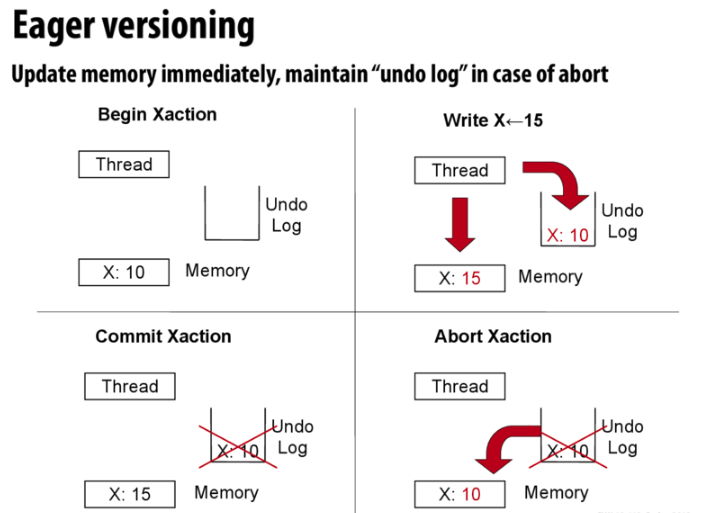
\includegraphics[scale=0.4]{Pictures/eager.png}
\caption{\textit{\color{gray}A simple example of eager version. \cite{Xelblade}.}}
\end{figure}

\begin{figure}[h!]
\centering
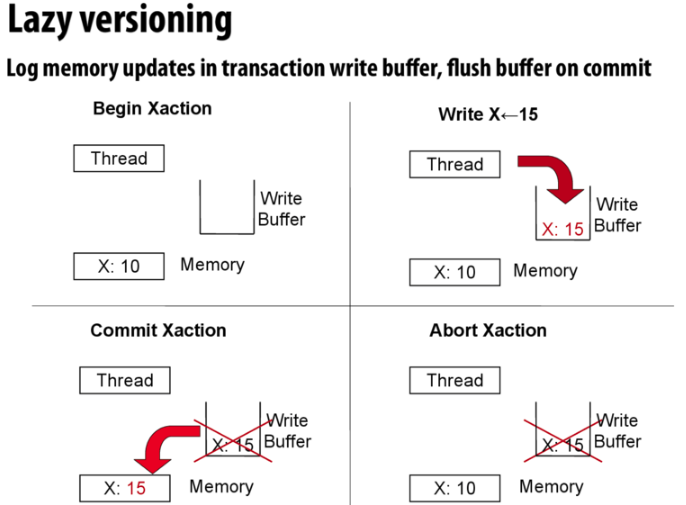
\includegraphics[scale=0.4]{Pictures/lazy.png}
\caption{\textit{\color{gray}A simple example of lazy version. \cite{Xelblade}.}}
\end{figure}

\subsection{Create transaction}
When the external program create an object of the transaction library, it's functions available to the transaction object. The transaction object able to pass the required values to send to the transaction library to make changes on them.

\subsection{Start transaction}
When the transaction start, the library store the version number associated with the data and a copy of the data itself into the library shared data set, to use later on to compare version numbers against each other, to determine the conflicts.

\subsection{Commit transaction}
This phase of the transaction, the library locks the used shared memory spaces in an atomic block, and hide from the other processes to write changes in to the local data set. After the changes has made on the local data set, before finalize the write process to the destination shared memory spaces, must to determine if any other process had accessed the same data set, and made changes on it. It is happening with compare the transaction version number associated with the shared memory space version number. 

\subsubsection{Version checking}
The version number representing the changes associated with destination data by the transactions. The transaction can detect the conflict early when first time accessing the value or when the transaction attempts to commit. When a transaction commit the changes, write the new values to the shared memory space, and the same time increasing the global version number to indicate the other transactions, that some changes happened with the value. At commit time or when accessing the value, the transaction compare the version numbers. The version number in the actual transaction and the global version number associated with the data must match. If the values are not the same the transaction will be cancelled, updating the local version number and rolling back the changes before writing the new value to the shared memory space and restart the transaction.

\subsubsection{Roll-back transaction}
The roll-back part of the transaction, simply goes back to the begging of the transaction and restart the process. The library should implement some sort of checking logic, that the roll-back process must be cancelled at some stage, otherwise it can create an infinite or very long looping time and cause starvation in the software application.

\subsubsection{Updating}
At commit time, if the compared versions are holding same values, then the transaction updating the shared memory space the target data set and closing the transaction. \\

The following code snippet is an atomic transaction to change nodes in linked list structure:
\begin{lstlisting}
atomic {
  int x = node.head;
  tail = node.tail;
}
\end{lstlisting}
\clearpage
\section{Target users}
The potential target users can be any programmer, how planning to use concurrent programming features in their application, but in the same time they wants to avoid of the lock based programming disadvantages. Since, STM provide interface to access the built in transactional functionalities through object accessible method call, it is easy to use because only need to include the library into the software application.\\

{\setlength{\parindent}{0cm}
The potential target users can be who:
\begin{enumerate}
\item Want to avoid of mutex and semaphore.
\item Want to use concurrent programming features.
\item Want to avoid deadlock and livelock.
\end{enumerate}
}


\section{Metrics}
The C++14 Software transactional Memory project is successful, when the library working as it is expected in all circumstances with no error accepted. To fulfil these achievement the project must produce the following requirements:


\textbf{Mandatory requirements:} 
\begin{enumerate}
\item The library have to:
	\begin{itemize}
	\item Full Software Transactional Memory implementation in C++ language.
	\item Full documentation of the library using Doxygen documentation tool.
	\item Tutorial showing how to use the library.
	\end{itemize}


\textbf{Discretionary requirements:} 

\item The library have to:
	\begin{itemize}
	\item Portable : tested across multiple platform (Windows, Linux, OSX).
	\item Web site: library backed up and demonstrating it usage.
	\end{itemize}

\clearpage
\textbf{Exceptional requirements:} 

\item The library have to:
	\begin{itemize}
	\item Benchmarked : The library fully benchmarked.
	\item Comparisons : Compare between other STM solutions and other approaches.
	\end{itemize}
\end{enumerate}

\subsubsection{FURPS}
As part of the metrics, the library should implement not functional requirements (FURPS)\cite{PPTX}
\begin{enumerate}
\item \textbf{Functionality} - Features, capabilities, security.
\item \textbf{Usability} - Human factors, help, documentation. 
\item \textbf{Reliability} - Frequency of failure, recoverability, predictability.
\item \textbf{Performance} - Response times, throughput, accuracy, availability,
resource usage. 
\item \textbf{Supportability} - Adaptability, maintainability, internationalization,
configurability. 
\end{enumerate}

`
\section{Other STM libraries}
The Software Transactional Memory was implemented in C/C++ language many time before. However, this project must produce a fully implemented STM library to support lock free transactions, possibly the library functionalities will be a bit restricted compare with the other C/C++ library implementations available. Why? Because those libraries are available years ago and developed over the time.\\

The Software Transactional Memory was implemented in many different languages as well, including C, C++, Clojure, Common Lisp, Haskell, Java, Python, Pearl and many more.

\clearpage
\textbf{Some C/C++ STM implementation:} 
\begin{enumerate}
\item TinySTM is a lightweight and efficient word-based STM implementation in C++.
\item libCMT based on Composed Memory Transaction written in C.
\item Intel STM Complier prototype Edition implements STM for C/C++ directly in a complier
\item stmmap based on shared memory accessing written in C.
\item TL2 transaction locking implementation of STM that’s been most widely accepted
\item CTL based on TL2 and added many extensions and optimization
\item many more
\end{enumerate}

\textbf{This project will be based on TL2 logics, which are the followings:}
\begin{enumerate}
\item Sample global version-clock.
\item Run through a speculative execution.
\item Lock the write-set.
\item Increment global version-clock.
\item Validate the read-set.
\item Commit and release the locks.
\end{enumerate}



\newpage
\section{Bibliography}
\begin{center}
\bibliographystyle{abbrv}
\bibliography{database.bib}

\end{center}


\end{document}